\section[Topologische Begriffe, Hilberträume, Fourierreihen]{Topologische Begriffe, Kompaktheit, Hilberträume, beschränkte Operatoren, Fourierreihen}
\Einleitung{Ihr geratet diese Woche mal wieder in einen regelrechten Vokabelsturm - immerhin seid ihr's inzwischen ja gewohnt.\\
Nehmt euch auch hier wieder genügend Zeit, um die Zusammenhänge gut zu verstehen, denn viele dieser Begriffe werden uns von nun an regelmäßig begleiten.\\
Die vielen Begriffe werden anschließend erweitert, um eine bestimmte Klasse von Basen euklidischer bzw. hermitescher Vektorräume zu definieren, die den Begriff der orthonormalen bzw. unitären Basen erweitern.\\
Die kurzfristige Motivation sind u. a. Fourierreihen - ein nützliches Werkzeug, um periodische Funktionen als Reihen darzustellen.}

\subsection{Toplogisches Vokabelgewitter}
Passt gut auf, denn die folgenden Begriffe werden für viele der folgenden Sätze beiläufig als Voraussetzungen gefordert, da wäre es schade, wenn ihr die nicht parat hättet!\\
Letztes Jahr hatte ich (Fabian) aufgrund einer weggefallenen Tutoriumsaufzeichnung hierzu ein \href{https://youtu.be/BPn-hFZh6ww}{Video auf YouTube} hochgeladen, in dem ich diesen Part erkläre. Vielleicht hilft's euch ja :)\\
Für vieles davon benötigen wir die offene Kugel, die wir uns letzte Woche schon in Bezug auf verschiedene Metriken angesehen hatten:
\begin{Wiederholung}
{Offene Kugel}
Die Teilmenge $\boxed{B_r(x):=\Menge{y\in X}{d(x,y)<r}\subseteq X}$ eines metrischen Raumes $(X,d)$ mit Abstandsfunktion $d$ heißt \red{offene Kugel} (manchmal auch \red{Ball}) mit Mittelpunkt $x$ und Radius $r$.
\end{Wiederholung}
\begin{Def}{Offene Teilmenge}
\begin{wrapfigure}{r}[0pt]{.35\textwidth}
 \vspace{-15pt}
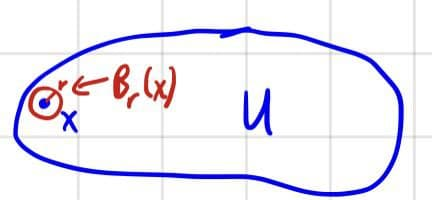
\includegraphics[width=.35\textwidth]{Dateien/06/06OffeneMenge.jpg}
 \vspace{-15pt}
\end{wrapfigure}
Wir nennen eine Teilmenge $U\subseteq X$ \red{offen}, wenn $\forall x\in U\,\exists r>0$, sodass $B_r(x)\subseteq U$.\\
\blue{Um jedes Element aus einer offenen Menge können wir also eine Kugel legen, die dann noch komplett in $X$ enthalten ist - egal wie nah wir an den Rand gehen!}
\end{Def}

\begin{Beispiel}{Das offene Intervall}
\begin{wrapfigure}{r}[0pt]{.15\textwidth}
 \vspace{-15pt}
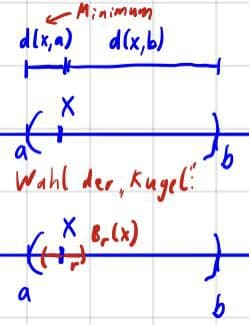
\includegraphics[width=.15\textwidth]{Dateien/06/06OffenIntervall.jpg}
 \vspace{-15pt}
\end{wrapfigure}
\Zz{Das offene Intervall $I=(a,b)$ mit $a,b\in\mathbb{R}$ ist offen.\footnote{Deswegen heißt es ja auch so. Aber wir wollen trotzdem einsehen, weshalb es unsere Definition für 'offen' erfüllt.}}
\Zb{Sei $x\in(a,b)$ beliebig.\\
Dann können wir als Radius $r$ unserer offenen Kugel $B_r(x)$ um $x$, die ja komplett in $I$ enthalten sein soll, einfach die Hälfte des Minimums der Abstände zu den Intervallgrenzen nehmen:
\begin{equation*}
    r:=\frac{1}{2}\min(d(x,a),d(x,b))=\frac{1}{2}\min(\Abs{x-a},\Abs{x-b}).
\end{equation*}
Also ist $I$ offen.}
\end{Beispiel}
\blue{Für das abgeschlossene Intervall $I_2=[a,b]$ funktioniert diese Konstruktion nicht mehr: Für $x=a$ wäre der Radius der Kugel $r=\min(\Abs{x-a},\Abs{x-b})=0$, was nicht erlaubt ist.\\
Für solche Fälle definieren wir:}
\begin{Def}
{Abgeschlossene Teilmenge}
Wir nennen eine Teilmenge $A\subseteq X$ \red{abgeschlossen}, wenn das Komplement $X\setminus A$ in $U$ offen ist.
\end{Def}
\begin{Beispiel}
{Die leere Menge ist sowohl offen als auch abgeschlossen}
Die leere Menge $\emptyset$ in einem metrischen Raum $X$ ist zum einen offen\footnote{da keine Elemente, um die man überhaupt Kugeln legen müsste} als auch abgeschlossen, denn das Komplement (der metrische Raum) ist als Teilmenge von sich selbst offen, weil die Kugeln um alle Punkte innerhalb des Raumes liegen müssen.\\
Also ist auch der metrische Raum selbst offen und abgeschlossen zugleich.
\end{Beispiel}

\begin{Beispiel}
{Merkwürdigkeiten bzgl. der diskreten Metrik}
Wir betrachten $\mathbb{R}$ mit der diskreten Metrik\footnote{Welche die Metrikaxiome erfüllt, denn\\
M1) ist offensichtlich erfüllt,\\
M2) ebenfalls (Symmetrie ist gegeben),\\
M3) können wir für die verschiedenen Fälle $x=y$ und $x\neq y$ zeigen: Für $x=y$ ist $0=d(x,y)\leq d(x,z)+d(y,z)\,\forall z$.\\
Für $x\neq y$ ist entweder $z\neq x$ oder $z\neq y$ oder beides. Also gilt ebenfalls $d(x,y)=1\leq d(x,z)+d(y,z).\,\checkmark$} $d(x,y):=\Cases{0&\tx{ für } x=y\\1&\tx{ sonst}}.$\\
Jede Teilmenge $T\subset \mathbb{R}$ ist offen. Betrachte als Beispiel $T=\MengeDirekt{5,\pi}\subset \mathbb{R}$, so können wir für $p\in T$ einfach offene Kugeln mit $r<1$ wählen, denn diese enthalten für jedes Element nur das Element selbst, weil ja $d(p,x)<r<1$ nur für $p$ selbst erfüllt ist.\\
Bezüglich dieser Metrik sind also alle Teilmengen von $\mathbb{R}$ zugleich offen als auch abgeschlossen.
\end{Beispiel}
\begin{Satz}
{Bemerkung}{Eigenschaften metrischer Räume}
Für einen metrischen Raum $(X,d)$ gelten folgende Aussagen:
\begin{itemize}
    \item Beliebige Vereinigungen offener Mengen sind offen.\footnote{Für jeden der Punkte muss es ja offene Kugeln geben, das überträgt sich bei der Vereinigung.}
    \item Beliebige Durchschnitte abgeschlossener Mengen sind abgeschlossen.
    \item \underline{Endliche} Durchschnitte offener Mengen sind offen.\footnote{Anschaulich kann man hierbei für Punkte des Durchschnitts einfach die kleinere von beiden Kugeln wählen.}
    \item Endliche Vereinigungen abgeschlossener Mengen sind abgeschlossen.
\end{itemize}
\end{Satz}
\begin{Def}
{Inneres}
Für eine Teilmenge $A\subseteq X$ nennen wir die Vereinigung aller offenen Teilmengen das \red{Innere $\mathring{A}$} von $A$, also $\mathring{A}=\bigcup_{B\subseteq A}B$.
\end{Def}

\begin{Def}
{Abschluss}
Für eine Teilmenge $A\subseteq X$ nennen wir den Durchschnitt aller abgeschlossenen Mengen, die $A$ enthalten, den \red{Abschluss $\Bar{A}$} von $A$, also $\Bar{A}=\bigcap_{B\supset A, B\tx{ abgeschl.}}B$.
\end{Def}
\begin{Def}
{Rand}
Die Differenz aus diesen beiden Mengen ist dann der \red{Rand $\partial A$} von $A$, also $\partial A=\Bar{A}\setminus \mathring{A}$.
\end{Def}
\begin{Beispiel}
{Teiloffenes Intervall}
Wir betrachten ein teiloffenes Intervall\footnote{Welches weder offen noch abgeschlossen ist!} $I:=[a,b)\subset \mathbb{R}$ mit $a,b\in\mathbb{R}$.\\
Dann sind Inneres, Abschluss und Rand von $I$ gegeben durch
\begin{equation*}
    \mathring{I}=(a,b),\quad \Bar{I}=[a,b],\quad \partial I=\MengeDirekt{a,b}.
\end{equation*}
\end{Beispiel}
\begin{Beispiel}
{Exotische Ränder}\label{beisp:06RationaleUndReelleZahlenAbschluss}
\Zz{Fassen wir $\mathbb{Q}\subset\mathbb{R}$ als Teilmenge von $\mathbb{R}$ auf, so ist $\partial\mathbb{Q}=\mathbb{R}$.}
\Zb{Dies habt ihr auf einem eurer ersten Übungsblätter bewiesen - die reellen Zahlen sind der Rand der rationalen Zahlen, da zwischen zwei reellen Zahlen $x,y$ mit $x<y$ stets eine rationale Zahl $q=\frac{m}{n}$ existiert.\footnote{Warum ist das dann gerade der Rand? Naja, das bedeutet, dass wir um keine reelle Zahl einen Ball legen können, der nicht auch Komponenten in den rationalen Zahlen hat.}\\
Dies kann man mit dem archimedischen Axiom beweisen:\\
Seien $x,y$ O.B.d.A. positiv mit $y>x$, so gibt es $n\in N$, sodass $(y-x)n>1$ ist. Ebenso gibt es $m\in \mathbb{N}$, sodass $\frac{m}{xn}>1$, aber $\frac{m-1}{xn}<1$ ist. Formen wir diese Relationen um, so haben wir
\begin{equation*}
    x<\frac{m}{n}<\frac{m-1}{n}+\frac{1}{n}<x+\frac{1}{n}<x+y-x=y
\end{equation*}
Also haben wir gezeigt, dass zwischen den reellen Zahlen $x$ und $y$ eine rationale Zahl der Form $q=\frac{m}{n}$ liegen muss.
}\\
Der Rand der leeren Menge ist stets die leere Menge selbst, $\partial\emptyset=\emptyset$.
\end{Beispiel}
\begin{Def}
{Abgeschlossene Kugel{,} Sphäre}
Die Menge $\Bar{B}_r(x)=\Menge{y\in\mathbb{R}^n}{d(x,y)\leq r}$ ist der Abschluss der offenen Kugel $B_r(x)$ im euklidischen $\mathbb{R}^n$.\\
Den Rand dieser Kugel $S_r(x):=\partial B_r(x)=\Menge{y\in\mathbb{R}^n}{d(x,y)=r}$ nennen wir \red{Sphäre} \blue{(anschaulich die Kugeloberfläche)}.
\end{Def}
\subsubsection{Einige Sätze zu den neuen Definitionen}
Eine wichtige erste Erkenntnis ist:
\begin{Satz}
{Satz}{Über stetige Abbildungen}
Für eine \underline{stetige} Abbildung $F:X\to Y$ zwischen metrischen Räumen gilt:
\begin{enumerate}
    \item Urbilder $F^{-1}(U)$ aller offenen Teilmengen $U\subseteq Y$ sind offen.
    \item Urbilder $F^{-1}(A)$ aller abgeschlossenen Teilmengen $A\subseteq Y$ sind abgeschlossen.
\end{enumerate}
Umgekehrt gilt: Erfüllt $F$ 1) oder 2), so ist $F$ stetig!
\end{Satz}
\begin{Satz}
{Satz}{Konvergenz in abgeschlossenen Teilmengen}
Genau dann, wenn $A\subseteq X$ abgeschlossen ist, liegt für jede konvergente Folge von \underline{Elementen aus $A$} der Grenzwert $x\in X$ ebenfalls in $A$.
\end{Satz}
Dieser Satz ist wichtig, denn darüber können wir die Vollständigkeit\footnote{in einem vollst. Raum konvergieren alle Cauchy-Folgen gegen Grenzwerte im Raum} und Abgeschlossenheit verknüpfen:
\begin{Satz}
{Satz}{Vollständigkeit und Abgeschlossenheit}
Für einen metrischen Raum $X$ und eine Teilmenge $A\subseteq X$ (mit derselben Metrik) gilt:
\begin{enumerate}
    \item $A$ ist vollständig $\implies$ $A$ ist abgeschlossen in $X$.
    \item $X$ ist vollständig und $A$ ist abgeschlossen $\implies$ $A$ ist vollständig.
\end{enumerate}
\end{Satz}

\subsubsection{Kompaktheit}
\begin{Def}
{Offene Überdeckung}
\begin{wrapfigure}{r}[0pt]{.12\textwidth}
 \vspace{-15pt}
\includegraphics[width=.11\textwidth]{Dateien/06/06KompakteÜberdeckung.jpg}
 \vspace{-15pt}
\end{wrapfigure}
Für einen metrischen Raum $X$ nennen wir eine Familie von offenen Teilmengen $(U_i)_{i\in I}$ ein \red{offene Überdeckung} von $A\subseteq X$, wenn $A$ in der Vereinigung dieser Mengen enthalten ist, d. h.\\
$A\subseteq \bigcup_{i\in I} U_i$.
\end{Def}
\begin{Def}
{Kompaktheit}
Falls wir zu \underline{jeder} offenen Überdeckung $(U_i)_{i\in I}$ von $A\subseteq X$ eine endliche Teilüberdeckung, d.h. eine Einschränkung der Indexmenge $I$ auf eine endliche Menge $J\subseteq I$ finden, sodass $(U_i)_{i\in J}$ immer noch eine offene Überdeckung von $A$ ist, so nennen wir $A\subseteq X$ \red{kompakt}.
\end{Def}
Wir werden sehen, dass man Kompaktheit für viele Räume auf Abgeschlossen- und Beschränktheit zurückführen kann.
\subsubsection{Einige verknüpfende Sätze}
Für die folgenden Sätze ist es nützlich, sich direkt Beispiele zu überlegen:
\begin{Satz}
{Satz}{Folgen in kompakten Mengen haben konvergente Teilfolgen}
Sei $A\subseteq X$ eine \underline{kompakte} Teilmenge eines metrischen Raumes.\\
Dann hat jede Folge in $A$ eine konvergente Teilfolge mit Grenzwert in $A$.\\
\blue{Es ist z. B. $I=[0,1]$ ein kompaktes Intervall.\footnote{Begründung: Siehe Satz von Heine-Borel.} jede beliebige Folge mit Zahlen aus $I$ hat also eine konvergente Teilfolge, deren Grenzwert in $I$ liegt.}
\end{Satz}
\begin{Satz}
{Folgerung}{Kompakte Teilmengen sind abgeschlossen und beschränkt}
Jede kompakte Teilmenge $A\subseteq X$ eines metr. Raumes ist \underline{abgeschlossen}, \underline{vollständig} und \underline{beschränkt}.
\end{Satz}
\begin{Satz}
{Satz}{Kompaktheit abgeschlossener Teilmengen}
Ist $X$ kompakt und ist $A\subseteq X$ abgeschlossen, so ist auch $A$ kompakt.
\end{Satz}

\begin{Satz}
{Satz}{Satz von Heine-Borel}
In jedem \underline{endlichdimensionalen}, \underline{normierten} \underline{Vektorraum} $V$\footnote{also insbesondere dem $\mathbb{R}^n$ mit der euklidischen Metrik} ist $A\subseteq V$ genau dann kompakt wenn $A$ abgeschlossen und beschränkt ist.\\
\blue{Jetzt ist auch klar, weshalb $I=[0,1]$ kompakt ist, denn es ist abgeschlossen und beschränkt.}
\end{Satz}
\begin{Satz}
{Satz}{Bild kompakter Mengen}
Sei $F:X\to Y$ eine \underline{stetige} Abbildung zwischen metrischen Räumen und $A\subseteq X$ eine \underline{kompakte} Teilmenge.\\
Dann ist das Bild $F(A)\subseteq Y$ kompakt.
\end{Satz}
Den folgenden Satz hatten wir schon als Spezialfall im letzten Semester kennengelernt:
\begin{Satz}
{Folgerung}{Minimum-Maximum-Eigenschaft}
\begin{wrapfigure}{r}[0pt]{.35\textwidth}
 \vspace{-15pt}
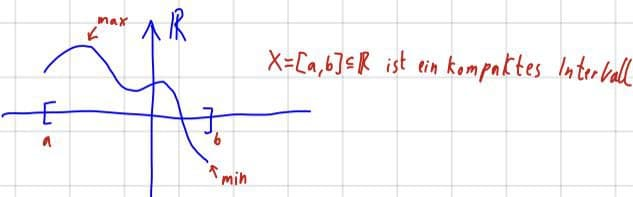
\includegraphics[width=.35\textwidth]{Dateien/06/06MinMax.jpg}
 \vspace{-15pt}
\end{wrapfigure}
Sei $f:X\to \mathbb{R}$ stetig und $X$ ein kompakter metrischer Raum.\\
Dann ist $f$ beschränkt und nimmt Minimum und Maximum \underline{in $X$} an.
\end{Satz}

\subsection{Funktionenfolgen}
Nun betrachten wir als Exkurs Folgen von stetigen Abbildungen $(F_n)_{n\in\mathbb{N}}$.\\
Dazu schauen wir uns an, welche Aussagen wir über deren Konvergenz gegen eine Grenzfunkion treffen können.\\
Es stellt sich heraus, dass wir hierfür zunächst einen stärkeren Stetigkeitsbegriff einführen müssen:
\begin{Def}
{Gleichmäßige Stetigkeit}
Wir nennen eine Abbildung $F:X\to Y$ zwischen metrischen Räumen \red{gleichmäßig stetig}, wenn \underline{für alle $x,x'\in X$} gilt, dass
\begin{equation*}
    d(F(x),F(x'))<\epsilon\tx{ falls } d(x,x')<\delta.
\end{equation*}
Dieses Kriterium fordert also ein bisschen mehr als die bekannte $\epsilon$-$\delta$-Stetigkeit.
\end{Def}
Zum Glück müssen wir nur die Stetigkeit der Abbildung testen, solange wir uns auf metrischen Räumen bewegen:
\begin{Satz}
{Satz}{Gleichmäßige Stetigkeit auf kompakten Räumen}
Jede \underline{stetige} Abbildung $F:X\to Y$ zwischen metrischen Räumen ist gleichmäßig stetig, falls $X$ kompakt ist.
\end{Satz}

Damit können wir nun mit den Funktionenfolgen durchstarten:
\begin{Def}
{Gleichmäßige Konvergenz}
Sind $(X,d_X)$ und $(Y,d_Y)$ metrische Räume und $(f_n:X\to Y)_{n\in\mathbb{N}}$ eine Folge von Abbildungen.\\
Wir sagen, dass $f$ genau dann \red{gleichmäßig} gegen eine Grenzfunktion $f$ \red{konvergiert}, wenn es für alle $\epsilon>0$ ein $N=N(\epsilon)\in\mathbb{N}$ gibt, sodass
\begin{equation*}
    d_Y(f_n(x),f(x))<\epsilon\quad \forall n\geq N\land \forall x\in X.
\end{equation*}
\end{Def}
\begin{Def}
{Punktweise Konvergenz}
Eine Folge $(f_n)$ von Abbildungen \red{konvergiert punktweise} gegen eine Abbildung $f$, falls $\lim_{n\to\infty}f_n(x)=f(x)\,\forall x\in X$.
\end{Def}
\begin{Satz}
{Satz}{Gleichmäßige Konvergenz impliziert punktweise Konvergenz}
Die Aussage steht im Titel; Gleichmäßige Konvergenz ist also eine stärkere Eigenschaft und nicht jede punktweise konvergente Folge konvergiert gleichmäßig.
\end{Satz}
Der grundlegende Unterschied zwischen der (intuitiveren) punktweisen und der gleichmäßigen Konvergenz ist, dass wir für die punktweise Konvergenz nur für jeden einzelnen Punkt $x\in X$ eine Grenzfunktion benötigen, die auch nicht unbedingt stetig sein muss.\\
Für gleichmäßige Konvergenz muss bei gegebenen $\epsilon$ ein $N$ existieren, sodass die Konvergenzbedingung $d(f_n(x),f(x))<\epsilon$ $\forall n\geq N$ tatsächlich \red{für alle} $x\in X$ erfüllt ist. Wir können also keine $x$-abhängigen Abschätzungen mehr machen.\\
\blue{Setzt euch genau mit den Beispielen aus dem Skript auseinander! Zudem folgen nun ein paar Beispiele, an denen die Unterschiede deutlich werden sollten:}
\begin{Beispiel}
    {Punktweise{,} aber nicht gleichmäßig konvergent (1/2)}
    Wir betrachten die Funktionenfolge:
    \begin{equation*}
        f_{n}: \mathbb{R} \longrightarrow \mathbb{R}, \qquad f_{n}(x)=nx\exp{(-nx^2)}
    \end{equation*}
    Ist die Folge punktweise konvergent? Dazu machen wir eine Fallunterscheidung und betrachten zuerst den Fall $x=0$. Hier ist die Sache klar:
    \begin{equation*}
        f_n(0) = 0 \,\xrightarrow[]{n\rightarrow\infty}\, 0
    \end{equation*}
    Für $x\neq 0$ benutzen wir den Satz über das exponentielle Wachstum:
    \begin{equation*}
        f_n(x)=\frac{nx}{\exp{(nx^2)}}=\frac{1}{x}\frac{nx^2}{\exp{(nx^2)}}=\frac{1}{x}\frac{y_n}{\exp{(y_n)}}\,\xrightarrow[]{n\rightarrow\infty\\\to y_n\to\infty}\,0
    \end{equation*}
    Die Folge ist also punktweise konvergent, da sie für jedes feste x konvergent ist. Aber heißt das auch, dass sie gleichmäßig konvergiert? \\
    Gleichmäßige Konvergenz bedeutet, dass $x$ nicht mehr fest ist, sondern beliebig variieren kann. Wir können also $x$ insbesondere durch eine Folge $x_n$ ersetzen, die wir frei bestimmen dürfen. Sollten wir eine Folge finden, die die Konvergenz der Funktionenfolge zerstört, wissen wir automatisch, dass sie nicht gleichmäßig konvergieren kann. In unserem Fall wird es sich als clever herausstellen, diese Folge durch
    \begin{equation*}
        x_n:=\frac{1}{n}\,\xrightarrow[]{n\rightarrow\infty}\, 0
    \end{equation*}
    festzulegen. Zur Erinnerung, die Definition der gleichmäßigen Konvergenz in Quantorenschreibweise (und mit dem Betrag als Abstand) lautet: 
    \begin{equation*}
        \forall \epsilon > 0 \,\exists N\in\mathbb{N}\, \forall x\in D_f \,\forall n\geq N: \quad \vert f_n(x)-f(x) \vert < \epsilon
    \end{equation*}
    Diese Aussage soll für alle x gelten, also setzen wir mal unsere Folge ein:
    \begin{equation*}
        \vert f_n(x_n)-f(x_n) \vert = \vert \frac{nx_n}{\exp{(nx_n^2)}} -0\vert = \exp\BracedIn{-\frac{1}{n}} \overset{\footnote{Durch die Monotonie der Exponentialfunktion gilt $\frac{1}{n}<1\implies -\frac{1}{n}>-1\implies \exp\BracedIn{-\frac{1}{n}}>\exp(-1)$}}{>} \exp{(-1)} = \frac{1}{e} 
    \end{equation*}
    Das sieht gar nicht gut aus, die Folge ist tatsächlich \red{nicht} gleichmäßig konvergent! Wenn wir nämlich ein $0<\epsilon < 1/e$ wählen, finden wir kein $N$ mehr, sodass die obige Bedingung erfüllt ist. \\
    Wie hat man sich das jetzt aber genau vorzustellen? Dazu betrachten wir die folgende Skizze:
    \begin{center}
        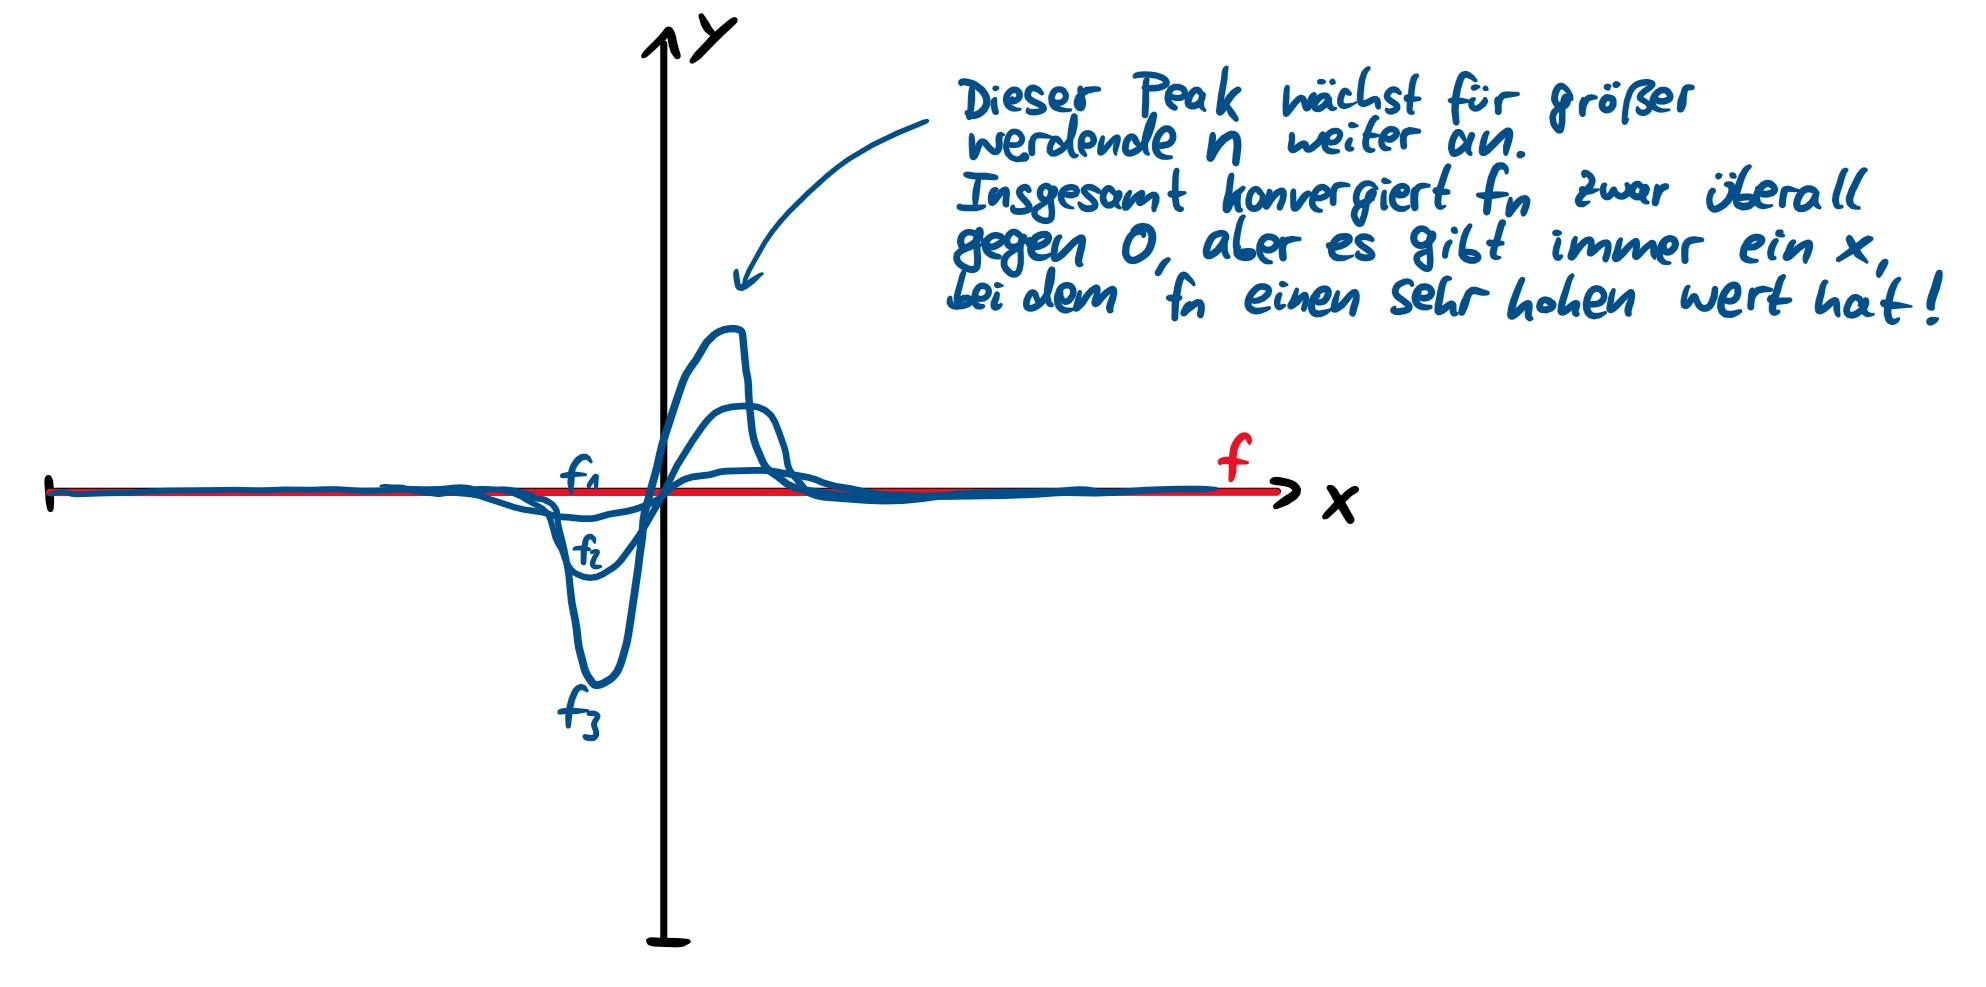
\includegraphics[width=.95\textwidth]{Dateien/06/06VeranschaulichungFunktionenfolgen.jpg}
    \end{center}
    Konvergiert eine Funktion punktweise aber nicht gleichmäßig, dann bedeutet das, dass sozusagen ein Teil der Funktion nicht konvergiert, dieser aber nicht fest ist und \glqq wandert\grqq. In der obigen Skizze baut sich zum Beispiel links und Rechts von der $y$-Achse ein Tal bzw. Berg auf, der zwar immer größer wird, aber auch immer weiter gegen die y-Achse wandert und somit in Bewegung ist. Somit konvergiert die Folge trotzdem in jedem Punkt separat, man muss nur genügend große $n$ wählen, sodass der Berg (oder das Tal) schon vorbei gewandert ist. Guckt man sich nun aber die Funktion als Ganzes an, so lassen sich die beiden Ausschläge nicht mehr wegdiskutieren. In unserem Fall haben wir eine Folge gewählt, die für jedes $n$ genau den Punkt heraussucht, der auf der Spitze des Berges liegt. Somit schauen wir uns bei jedem $n$ genau die \glqq Problemstelle\grqq~an und erhalten so eine nicht konvergierende Folge. \\
    Diese Beschreibung ist natürlich sehr salopp und nicht präzise formuliert, hilft aber hoffentlich, sich das Phänomen besser vorstellen zu können. Es ist wirklich nur zu empfehlen, mal eine Weile darüber nachzudenken, dann ist das auch nicht mehr so schwer ;)
\end{Beispiel}

\begin{Beispiel}
    {Nun aber auch mit gleichmäßiger Konvergenz (2/2)}
    Wir betrachten die Funktionenfolge
    \begin{equation*}
        f_n(x)=\sqrt{\vert x \vert^2 + \frac{1}{n^2}} \qquad x \in \mathbb{R}.
    \end{equation*}
    Konvergiert diese Folge gleichmäßig gegen eine Grenzfunktion, sagen wir $f(x)=\vert x \vert$? In weiser Voraussicht und um die weitere Rechnung plausibel zu machen, schauen wir uns zunächst die folgende Ungleichung an: 
    \begin{equation*}
        \sqrt{a+b} \leq \sqrt{a+b+2\sqrt{ab}} = \sqrt{(\sqrt{a}+\sqrt{b})^2}=\sqrt{a}+\sqrt{b}.
    \end{equation*} \\
    
    Damit können wir nun recht schnell nachprüfen:
    \begin{align*}
        \forall \epsilon > 0 \,\exists N\in\mathbb{N}\, &\forall x\in D_f \,\forall n\geq N: \\
            &\vert f_n(x)-f(x) \vert = \bigl| \sqrt{\vert x \vert^2 + \frac{1}{n^2}} - \vert x \vert \bigr| \leq \bigl| \vert x \vert + \frac{1}{n} - \vert x \vert \bigr| = \frac{1}{n} \leq \frac{1}{N} < \epsilon
    \end{align*}
    Das Kriterium ist also erfüllt und die Funktion damit gleichmäßig konvergent (und daher auch automatisch punktweise konvergent). Im Gegensatz zum vorherigen Beispiel geht die Sache hier auf, da wir die $x$-Abhängigkeit in der Abschätzung losgeworden sind.
\end{Beispiel}
\blue{Anmerkung: Bei gleichmäßiger Konvergenz von $f_n$ gegen eine Grenzfunktion $f$ gilt:
\begin{equation*}
    \int_a^{b} f(x) \text{d}x = \lim_{n\rightarrow \infty} \int_a^{b} f_n(x) \text{d}x 
\end{equation*}
Es lassen sich also Integral und Limes vertauschen. Das ist im Allgemeinen nicht selbstverständlich, in der Physik aber oft notwendig. In Mathe 3 lernt ihr Sätze mit schwächeren Bedingungen als gleichmäßige Konvergenz kennen, die eine solche Vertauschung rechtfertigen (zum Beispiel den Satz über die majorisierte Konvergenz).
}

\subsection{Vollständige Vektorräume: Jeder Hilbert ist ein Banach}
\begin{Wiederholung}{Cauchy-Folge}
Wir nennen eine Folge $(x_n)$ \red{Cauchy-Folge}, wenn für große $n$ die Abstände der Folgenglieder zueinander beliebig klein werden, d.h.
\begin{equation}
    \forall\varepsilon>0\,\exists N(\varepsilon)\in\mathbb{N}:\quad \forall m, n \geq N:\quad d(x_m, x_n)<\varepsilon.
\end{equation}
\end{Wiederholung}
\begin{Wiederholung}{Metrischer Raum}
Einen \underline{metrischen Raum} ($X, d$)\footnote{Eine Menge $X$ mit der Metrik/Abstandsfunktion $d$}, in dem \underline{alle} Cauchy-Folgen gegen Werte aus dem Raum konvergieren, nennen wir \red{vollständig}.
\end{Wiederholung}
\blue{Die reellen Zahlen waren vollständig, die rationalen Zahlen nicht.}
\begin{Def}
{Banachraum}
Einen \underline{vollständigen}\footnote{bezüglich der von der Norm induzierten Metrik}, \underline{normierten} Vektorraum nennen wir von nun an \red{Banachraum}.
\end{Def}
\begin{Def}
{Hilbertraum}
Einen reellen oder komplexen Vektorraum mit einem \underline{Skalarprodukt}, der  \underline{vollständig}\footnote{bezüglich der vom Skalarprodukt induzierten Metrik} ist, nennen wir von nun an \red{Hilbertraum}.
\end{Def}
\begin{Satz}
{Bemerkung}{Jeder Hilbert ist ein Banach}
Da durch das Skalarprodukt $\BiFo{\cdot, \cdot}$ auch immer eine Norm $\Norm{v}=\sqrt{\BiFo{v,v}}$ und dadurch wiederum eine Metrik $d(v,w)=\Norm{v-w}=\sqrt{\BiFo{v-w,v-w}}$ induziert wird, ist jeder Hilbertraum auch ein Banachraum.
\end{Satz}
Der folgende Satz zeigt uns, weshalb es wichtig war, einzusehen, dass auf endlichdimensionalen Vektorräumen alle Normen äquivalent sind.
\begin{Satz}
{Satz}{Äquivalente Normen und Cauchy-Folgen}
Sind $\Norm{\cdot}_1$ und $\Norm{\cdot}_2$ zwei äquivalente Normen auf $V$, so ist eine Folge $(x_n)\in V$ bzgl. der durch $\Norm{\cdot}_1$ induzierten Metrik $d_1$ genau dann eine Cauchy-Folge, wenn sie bzgl. der durch $\Norm{\cdot}_2$ induzierten Metrik $d_2$ eine ist.
\end{Satz}
Es ist also unter vielen Umständen egal, durch welche Norm wir eine Folge betrachten.

\subsection{Beschränkte Operatoren und die Operatornorm}
\blue{Wir schauen uns nun wieder lineare Abbildungen\footnote{d. h. $F(\lambda v+w)=\lambda F(v)+F(w)$ für alle $v,w\in V_1,\lambda\in \mathbb{K}$.} $F:V_1\to V_2$ zwischen \underline{normierten} Vektorräumen $V_1$ und $V_2$ an.}
\begin{Def}
{Beschränktheit}
Wir nennen eine lineare Abbildung $F:V_1\to V_2$ zwischen normierten Vektorräumen $(V_1,\Norm{\cdot}_1)$, $(V_2,\Norm{\cdot}_2)$ \red{beschränkt}, falls eine Konstante $C\geq 0$ existiert, sodass
\begin{equation}
    \Norm{F(u)}_2\leq C\Norm{u}_1\quad\forall u\in V_1,
\end{equation}
das Bild darf uns im Bildraum also nicht abhauen.\\
Meistens ist man nur an der kleinstmöglichen Konstante\footnote{wir erinnern uns, dass das Supremum die kleinste obere Schranke war.} interessiert und formt die Bedingung daher um:\footnote{wobei man $u$ mit $\Norm{u}_1=0$ herausnimmt, damit man nicht durch 0 teilt.}
\begin{equation}
    \iff \sup_{u\in V_1\setminus\MengeDirekt{0}}\frac{\Norm{F(u)}_2}{\Norm{u}_1}\leq C<\infty.
\end{equation}
\end{Def}

\begin{Def}
{Operatornorm}
Nutzt man die Linearität von $F$ aus, kann man dies noch etwas handlicher gestalten:
\begin{eqnarray*}
    \Norm{F}&:=&\sup_{u\in V_1\setminus\MengeDirekt{0}}\frac{\Norm{F(u)}_2}{\Norm{u}_1}\overset{\footnote{Wir definieren den Einheitsvektor in $u$-Richtung als $x$ und setzen mit $\Norm{u}_1=:c$ einfach $u=c\cdot x$ ein.}}{=}\sup_{x\in V_1:\Norm{x}_1=1}\frac{\Norm{F(cx)}_2}{\Norm{cx}_1}\\
    &\overset{\footnote{Linearität}}{=}&\sup_{x\in V_1:\Norm{x}_1=1}\frac{\Norm{cF(x)}_2}{\Norm{cx}_1}\overset{\footnote{Homogenität der Norm}}{=}\sup_{x\in V_1:\Norm{x}_1=1}\frac{\Abs{c}\Norm{F(x)}_2}{\Abs{c}\Norm{x}_1}\\
    &\overset{\footnote{weil wir $x$ als Einheitsvektor definiert hatten, ist $\Norm{x}_1=1$}}{=}&\sup_{x\in V_1:\Norm{x}_1=1}\Norm{F(x)}_2.
\end{eqnarray*}
Dies nennen wir die \red{Operatornorm} von $F$, also
\begin{equation}
    \boxed{\Norm{F}:=\sup_{x\in V_1:\Norm{x}_1=1}\Norm{F(x)}_2}.
\end{equation}
\end{Def}
Hiermit können wir die Bedingung für Beschränktheit umschreiben:\\
$F$ beschränkt $\iff$ $\Norm{F}<\infty$.\\
\blue{Die Operatornorm können wir uns für den $\mathbb{R}^2$ tatsächlich ziemlich gut bildlich vorstellen:}
\begin{Beispiel}{Operatornorm im $\mathbb{R}^2$}
Wir betrachten $F:\mathbb{R}^2\to\mathbb{R}^2,\,F(x,y)=\MatrixInline{2x\\4y}$, wobei $\mathbb{R}^2$ mit der euklidischen Norm versehen sei.\\
Dann ist
\begin{equation*}
    \Norm{F}=\sup_{\Norm{v}=1}\Norm{F(v)}=\sup_{\Norm{v}=1}\sqrt{4x^2+16y^2}\leq\sqrt{16}\sup_{\Norm{v}=1}\sqrt{x^2+y^2}=4\sup_{\Norm{v}=1}\Norm{v}=4.
\end{equation*}
Dies ist die kleinste obere Schranke, denn für $v=\MatrixInline{0\\1}$ (mit $\Norm{v}=1$ ist $\Norm{F(v)}=\sqrt{4\cdot0^2+16}=4$, das Supremum wird also angenommen.\\
\begin{wrapfigure}{r}[0pt]{.35\textwidth}
 \vspace{-15pt}
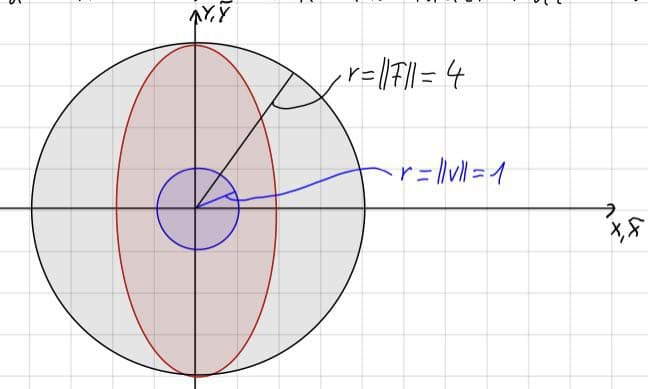
\includegraphics[width=.35\textwidth]{Dateien/06/06OperatornormBeispiel.jpg}
 \vspace{-15pt}
\end{wrapfigure}
\textbf{Bildliche Vorstellung}:\\
In dieser Darstellung betrachten wir aus dem Urbildraum alle Vektoren\footnote{als Punkte in der $\mathbb{R}^2$-Ebene} $v$ mit $\Norm{v}=1$, d. h. Punkte, für die $\sqrt{x^2+y^2}=1\iff x^2+y^2=1$ gilt. Es handelt sich also um den Einheitskreis.\\
Stecken wir diese Bedingung in $F$, so landen wir nach Umformung von $F(x,y)=\MatrixInline{2x\\4y}=:\MatrixInline{\Tilde{x}\\\Tilde{y}}\iff\MatrixInline{x\\y}=\MatrixInline{\Tilde{x}/2\\\Tilde{y}/4}$ bei $\BracedIn{\Tilde{x}/2}^2+\BracedIn{\Tilde{y}/4}^2=1$.\\
Dies ist eine Ellipse mit den Halbachsen 2 und 4!\\
Die Operatornorm ist dann anschaulich der Radius des Kreises, der alle Bildpunkte beschränkt.
\end{Beispiel}
\begin{Satz}
{Satz}{Lineare Abbildungen zwischen endlichdimensionalen Vektorräumen}
Lineare Abbildungen zwischen endlichdimensionalen Vektorräumen $(V_1,\Norm{\cdot}_1)$ und $(V_2,\Norm{\cdot}_2)$ sind beschränkt.\\
Der Beweis ist nicht im Skript, aber insofern interessant, als dass er den Nutzen äquivalenter Normen noch einmal hervorhebt.\\
\Zb{Ansatz: Sei $\dim V_1=n$ und $F:V_1\to V_2$ linear.\\
Dann können wir für eine beliebige Basis $B_1=(b_1,\ldots,b_n)$ von $V_1$ $v\in V_1$ als Linearkombination\footnote{mit Koeffizienten $\mu_i$} aufschreiben:\\
$v=\sum_{i=1}^n\mu_i b_i$.\\
Wir definieren nun $\Norm{v}_S:=\sum_{i=1}^n\Abs{\mu_i}$ als Norm.\footnote{Wieso gerade diese? Das wird in der Abschätzungskette deutlich, denn so können wir die Äquivalenz gut ausnutzen.}\\
Da $V_1$ endlichdimensional ist, sind die Normen äquivalent ($\Norm{\cdot}_S\sim\Norm{\cdot}_1$), d. h., es gibt $M>0$, sodass $\Norm{v}_s<M\Norm{v}_1$ (i).\\
Daher gilt die Abschätzungskette
\begin{eqnarray*}
    \Norm{F(v)}_2&=&\Norm{F\BracedIn{\sum_{i=1}^n\mu_ib_i}}_2\overset{\footnote{Linearität von $F$}}{=}\Norm{\sum_{i=1}^n\mu_iF(b_i)}_2\\
    &\overset{\footnote{Dreiecksungleichung und Linearität der Norm}}{\leq}&\sum_{i=1}^n\Abs{\mu_i}\Norm{F(b_i)}_2\leq \BracedIn{\sum_{i=1}^n\Abs{\mu_i}}n\max_{k\in\MengeDirekt{1,\ldots,n}}\Norm{F(b_k}_2\\
    &\overset{\footnote{Das Maximum einer endlichen Menge ist endlich, weshalb wir definieren können $m:=n\max_{k\in\MengeDirekt{1,\ldots,n}}\Norm{F(b_k)}_2$. Zudem ist ja $\sum_{i=1}^n\Abs{\mu_i}=\Norm{v}_s$}}{=}&m\Norm{v}_s\overset{\tx{(i)}}{\leq}m\cdot M\Norm{v}_1.
\end{eqnarray*}
Mit $C:=m\cdot M$ ist $F$ also beschränkt ($\Norm{F(v)}_2\leq C\Norm{v}$).}
\end{Satz}
\begin{Satz}
{Satz}{Stetigkeit und Beschränktheit}
Für eine lineare Abbildung $F:V_1\to V_2$ zwischen normierten Vektorräumen $(V_1,\Norm{\cdot}_1)$ und $(V_2,\Norm{\cdot}_2)$ gilt:
\begin{equation}
    \boxed{F\tx{ beschränkt }\iff F\tx{ stetig}}.
\end{equation}
\end{Satz}

\begin{Def}
{Stetige Abbildungen}
Für zwei metrische Räume $X$ und $Y$ definieren wir die \red{Menge der stetigen Abbildungen} von $X\to Y$:
\begin{equation}
    C(X,Y):=\Menge{f:X\to Y}{f\tx{ stetig}}.
\end{equation}
\end{Def}
\begin{Def}
{Maximumsmetrik}
Sei nun $X$ \underline{kompakt}, so ist durch $d_\infty: C(X,Y)\times C(X,Y)\to [0,\infty),$\\$d_\infty(f,g):=\max_{x\in X}d_Y(f(x),g(x))$ eine Metrik definiert.
\end{Def}
\begin{Beispiel}
{Anschauung der Maximumsmetrik}
\begin{wrapfigure}{r}[0pt]{.25\textwidth}
 \vspace{-15pt}
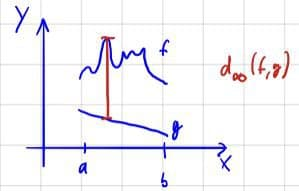
\includegraphics[width=.25\textwidth]{Dateien/06/06Maximumsmetrik.jpg}
 \vspace{-15pt}
\end{wrapfigure}
Sei $X=[a,b],\, Y=\mathbb{R}$ mit der Betragsmetrik.\\
Anschaulich ist dann der Abstand zwischen zwei Funktionen $f,g\in C(X,Y)$ leicht zu verstehen, wir haben das mal aufgemalt.\\
Abstrakt ist vielleicht noch das Konzept, dass wir Abbildungen überhaupt einen Abstand zuordnen.
\end{Beispiel}

\begin{Satz}
{Satz}{Vollständigkeit des Raumes der stetigen Abbildungen}
Ist ein metr. Raum $X$ \underline{kompakt} und $Y$ ein \underline{vollständiger} metr. Raum, so ist $(C(X,Y),d_\infty)$ ein vollständiger metrischer Raum.
\end{Satz}



\subsection{Hilbertbasen - das Werkzeug für unendlichdimensionale, separable Vektorräume}
\subsubsection{Sind wir noch ganz dicht? Der Weg zur Separabilität}
\begin{Def}
{Dichtheit}
Für einen metrischen Raum $(X,d)$ nennen wir eine Teilmenge $Y\subseteq X$ \red{dicht in $X$}, wenn der Abschluss von $Y$ gleich $X$ ist, also $\Bar{Y}=X$.\\
Dies ist äquivalent zur folgenden Darstellung:
\begin{equation}
    \forall x\in X,\, \forall\epsilon>0\,\exists y\in Y,\tx{ sodass } d(x,y)<\epsilon.
\end{equation}
\end{Def}
\begin{Wiederholung}
{Abzählbarkeit}
Wir nennen eine nicht-leere Menge $A$ \red{abzählbar}, falls es eine \underline{surjektive}\footnote{es wird also auf alle Elemente aus $A$ abgebildet} Abbildung $\varphi$ aus den natürlichen Zahlen nach $A$ gibt, d.h. $\varphi:\mathbb{N}\to A$ surjektiv.\\
Existiert diese Abbildung nicht, so nennen wir $A$ \red{überabzählbar}.
\end{Wiederholung}
\begin{Def}
{Separabilität}
Falls für $(X,d)$ eine \underline{dichte} Teilmenge existiert, die \underline{abzählbar} ist, nennen wir $X$ \red{separabel}.
\end{Def}

\begin{Beispiel}
{Rationale und reelle Zahlen (1/2)}
Die rationalen Zahlen $\mathbb{Q}$ liegen dicht in $\mathbb{R}$, denn wir hatten in \hyperref[beisp:06RationaleUndReelleZahlenAbschluss]{Beispiel 6.5} gesehen, dass $\partial \mathbb{Q}=\mathbb{R}$.\\
Da $\mathbb{Q}$ abzählbar ist, ist der $\mathbb{R}^1$ separabel.\\
Zudem liegt der $\mathbb{Q}^n$ ebenfalls dicht in $\mathbb{R}^n$, somit ist auch der $\mathbb{R}^n$ separabel.
\end{Beispiel}

\begin{Beispiel}
{Polynome und stetige Funktionen (2/2)}
Auf einem kompakten Intervall liegt die Menge der Polynome dicht in der Menge der stetigen Funktionen.\\
Auf solchen Intervallen lassen sich stetige Funktionen also beliebig gut durch Polynome approximieren!\\
Falls ihr Interesse am Beweis habt, ist das der \href{https://de.wikipedia.org/wiki/Satz_von_Stone-Weierstra\%C3\%9F}{Satz von Stone-Weierstraß}.
\end{Beispiel}

\subsubsection{Hilbertbasen als Spezialfall orthonormaler Familien}
\begin{Def}
{Orthogonale Familien}
Für eine Bilinear- oder hermitesche Form $\BiFoLeer$ auf einem $\mathbb{K}$-Vektorraum nennen wir eine Teilmenge $U\subseteq V$ von Vektoren \red{orthonormale Familie}, falls $\BiFo{u,u}=1$ und $\BiFo{u,v}=0\,\forall u,v\in V,\,u\neq v$.
\end{Def}
\begin{Satz}{Satz}
{Abzählbarkeit orthonormaler Familien}
Auf einem \underline{separablen} euklidischen\footnote{es existiert also ein reelles Skalarprodukt} oder hermiteschen\footnote{es existiert also ein komplexes Skalarprodukt} Vektorraum ist \underline{jede} orthonormale Familie $(v_i)_{i\in I}$ von Vektoren abzählbar.\footnote{Die Indexmenge $I$ ist somit auch abzählbar.}
\end{Satz}

\begin{Satz}
{Satz}{Besselsche Ungleichung}
Für eine abzählbare orthonormale Familie $(v_i)_{i\in I}$ auf $V$\footnote{eukl. oder herm.} gilt, dass für jeden Vektor $x\in V$ die Summe der Projektionen auf die $v_i$ durch die Norm von $x$ beschränkt ist:
\begin{equation}
    \sum_{i\in I}\Abs{\BiFo{x,v_i}}^2\leq\Norm{x}^2.
\end{equation}
Ist $V$ vollständig, so konvergiert die Reihe $\sum_{i\in I}\BiFo{x,v_i}v_i=x_\infty$.\\
Ist dieser Grenzwert $x_\infty=x$, so gilt Gleichheit, $\sum_{i\in I}\Abs{\BiFo{x,v_i}}^2=\Norm{x}^2$.
\end{Satz}
\begin{Def}
{Hilbertbasis}
Falls jeder Vektor $x\in V$ sich als Reihe $x=\sum_{i\in I}\BiFo{x,v_i}v_i$ darstellen lässt, wobei $(v_i)_{i\in I}$ wieder eine abzählbare orthonormale Familie sei, nennen wir $(v_i)_{i\in I}$ eine \red{Hilbertbasis} von $V$.
\end{Def}
\blue{Dies erweitert den Basisbegriff\footnote{genauer: den der orthonormalen/unitären Basis} auf unendlichdimensionale Vektorräume.\\
Man kann sich die Reihe sozusagen als unendliche, aber abzählbare Linearkombination vorstellen.}

\begin{Satz}
{Satz}{Zur Hilbertbasis}
Für eine abzählbare orthonormale Familie $B=(b_1,b_2,\ldots)$ auf $V$ sind äquivalent:
\begin{enumerate}
    \item $\Spann{b_1,b_2,\ldots}$ ist dicht in $V$.\\
    \blue{Jedes Element von $V$ lässt sich durch Linearkombinationen von Vektoren aus $B$ beliebig gut approximieren.}
    \item $B$ ist eine Hilbertbasis.\\
    \blue{Für alle $x\in V$ gilt: $x=\sum_i\BiFo{x,v_i}v_i$.}
    \item $\forall x,y\in V$ gilt: $\BiFo{x,y}=\sum_{k}\BiFo{x,b_k}\overline{\BiFo{y,b_k}}$.
    \item $\forall x\in V$ gilt:
    \begin{equation}
        \Norm{x}^2=\sum_k\Abs{\BiFo{x,v_k}}^2.
    \end{equation}
    Dies ist bekannt als die \red{parsevalsche Gleichung}.
\end{enumerate}
\end{Satz}
\blue{Falls das alles jetzt noch sehr abstrakt ist: Keine Angst, Anwendungen finden sich mit Fourierreihen im nächsten Kapitel.}

\subsection{Fourierreihen - die perfekte Welle?}
\subsubsection{Physikalische Motivation}
\begin{wrapfigure}{r}[0pt]{.35\textwidth}
 \vspace{-15pt}
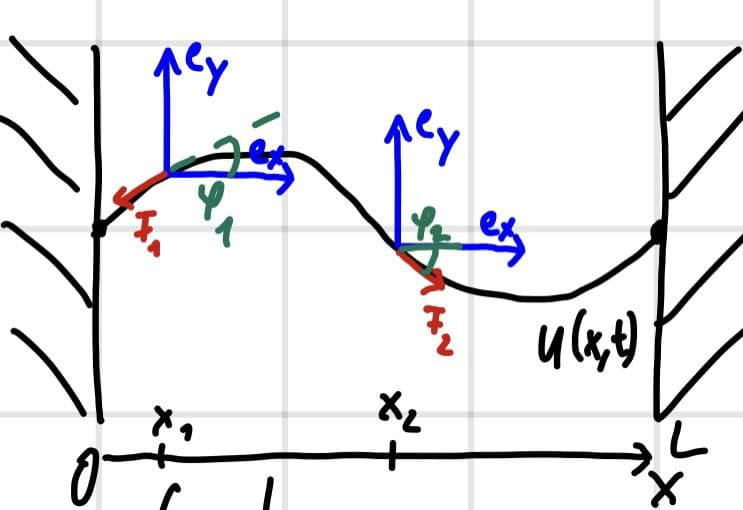
\includegraphics[width=.35\textwidth]{Dateien/06/06Saite.jpg}
 \vspace{-15pt}
\end{wrapfigure}
\blue{Wir betrachten eine an zwei Enden fest eingespannte Saite. Wird sie ausgelenkt, so beginnt sie zu schwingen. Nehmen wir an, dass die Saite nur transversal schwingt, so können wir die Auslenkung in $y$-Richtung durch $u(x,t)$ mit $x\in (0,L)$ und $u(0,t)=u(L,t)=0$ beschreiben. Wir betrachten nun die wirkenden Kräfte:\\
Die Tangentialkräfte an zwei beliebigen Punkten $x_1$ und $x_2$ müssen sich horizontal ausgleichen, d. h. (mit $\Fvec_i$ als den Tangentialvektor der Funktion an der Stelle $i$)
\begin{equation*}
    \Norm{\Fvec_1}\cos\varphi_1=\Norm{\Fvec_2}\cos\varphi_2=:S.
\end{equation*}
Dies bezeichnen wir im Folgenden als Spannkraft $S$.\\
Zudem ist die vertikale Kraft $V$ gegeben durch
\begin{equation*}
    V=V_1+V_2=-\Norm{\Fvec_1}\sin \varphi_1+\Norm{\Fvec_2}\sin\varphi_2.
\end{equation*}
Um weitere Aussagen treffen zu können, bilden wir den Quotienten $\frac{V}{S}$ und haben
\begin{align*}
    \frac{V}{S}&=\frac{-\Norm{\Fvec_1}\sin \varphi_1+\Norm{\Fvec_2}\sin\varphi_2}{\Norm{\Fvec_1}\cos\varphi_1}=-\frac{-\Norm{\Fvec_1}\sin \varphi_1}{\Norm{\Fvec_1}\cos \varphi_1}+\frac{\Norm{\Fvec_2}\sin \varphi_2}{\Norm{\Fvec_2}\cos \varphi_2}\\
    &=\tan\varphi_2-\tan\varphi_1=\diffp{u(x_2,t)}{x}-\diffp{u(x_1,t)}{x},
\end{align*}
weil $\tan\varphi_i$ gerade die Steigung der Saite an der Stelle $i$ beschreibt.\\
Andererseits ergibt sich die vertikale Kraft auch ganz klassisch durch
\begin{equation*}
    V=m a= \rho(x_2-x_1) a=\rho(x_2-x_1)\diffp{^2u(x,t)}{t^2},
\end{equation*}
wobei wir $m=\rho \Delta x$ mit der Längenmassendichte $\rho$ angesetzt haben.\\
Setzen wir diese Gleichung in $\frac{V}{S}$ ein, so ergibt sich
\begin{align*}
    \frac{\rho(x_2-x_1)}{S}\diffp{^2u(x_2,t)}{t^2}&=\diffp{u(x_2,t)}{x}-\diffp{u(x_1,t)}{x}\\
    \iff \diffp{^2u(x,t)}{t^2}&=\frac{S}{\rho}\frac{\diffp{u(x_2,t)}{x}-\diffp{u(x_1,t)}{x}}{x_2-x_1}\overset{x_2\to x_1}{\longrightarrow}\frac{S}{\rho}\diffp{^2u(x,t)}{x^2}.
\end{align*}
Wir haben hiermit die sogenannte Wellengleichung hergeleitet: $\boxed{\diffp{^2u(x,t)}{t^2}=\frac{S}{\rho}\diffp{^2u(x,t)}{x^2}}$ (mit $S,\rho>0$).\\
Dies ist mit den Randbedingungen $u(0,t)=u(L,t)=0$ ein homogenes Randwertproblem, für das sich\footnote{mit noch nicht behandelten Techniken} Lösungen finden lassen.\footnote{Exkurs: Der Ansatz ist eine Separation, also $u(x,t)=v(x)w(t)$. Dann ist nämlich $\frac{S}{\rho}\frac{v''(x)}{v(x)}=\frac{\Ddot{w}(t)}{w(t)}=const.$, da wir ja $x$ und $t$ separat variieren können. Damit ist $v''(x)+\lambda v(x)=0$ und analog $\Ddot{w}(t)+\frac{\rho}{S}w(t)=0$. Die Lösungen können dann separat gefunden werden.}
Tatsächlich findet man (der Einfachheit halber mit $L=\pi$), dass Funktionen mit $u(x,t)=\sin(kx)\cos(\sqrt{\frac{S}{\rho}}kt)$ und $u(x,t)=\sin(kx)\sin(\sqrt{\frac{S}{\rho}}kt)$ diese Gleichung lösen, wobei $k\in \mathbb{Z}$ aus den Randbedingungen kommt.\\
Weil wir dieses für die Lösungen aber beliebig wählen können und\footnote{weil wir eine lineare DG betrachten} auch Linearkombinationen\footnote{anschaulich: Überlagerungen von Wellen} eine Lösung darstellen, muss auch
\begin{equation*}
    u(x,t)=\sum_{k=1}^\infty \sin(kx)\BracedInSqr{a_k\cos\BracedIn{\sqrt{\frac{S}{\rho}}kt}+b_k\sin\BracedIn{\sqrt{\frac{S}{\rho}}kt}}
\end{equation*}
eine Lösung sein. Physikalisch entspricht das der Überlagerung verschiedener Wellen mit unterschiedlichen Frequenzen.}\\
Die Frage ist nun, wie wir das verallgemeinern können. Welche Art von Funktionen können wir in dieser Form darstellen?
\subsubsection{L-Periodische Funktionen}
\begin{Def}
{Periodische Funktion}
Wir nennen eine Funktion $f:\mathbb{R}\to\mathbb{K}$ (mit $\mathbb{K}=\mathbb{R}$ oder $\mathbb{K}=\mathbb{C}$) \red{periodisch} mit Periode $L>0$, wenn
\begin{equation*}
    f(x+L)=f(x)\quad \forall\, x\in\mathbb{R}.
\end{equation*}
\end{Def}
Weil wir schon Funktionen wie $\sin x$, $\cos x$ und $\exp (ix)$ kennen, die $2\pi$-periodisch sind, betrachten wir nun nur noch solche.\\
Durch Reskalierung können wir wieder zurück zur $L$-Periodizität kommen: $F(x)=f\BracedIn{\frac{2\pi}{L}}$ ist $L$-periodisch, wenn $f$ $2\pi$-periodisch ist.
\begin{Beispiel}
{Periodizität durch Reskalierung}
\begin{itemize}
    \item $f_1(x)=e^{ix}=\overbrace{e^{2\pi i}}^{=1}e^{ix}=e^{i(x+2\pi)}=f_1(x+2\pi)$ ist periodisch mit $L=2\pi$.
    \item $f_2(x)=e^{i\frac{2\pi x}{5}}=e^{2\pi i}e^{i\frac{2\pi x}{5}}=e^{i\frac{2\pi}{5}(x+5)}=f_2(x+5)$ ist periodisch mit $L=5$.
\end{itemize}
\end{Beispiel}
\begin{Def}
{Vektorraum der $2\pi$-periodischen Funktionen}
Wir definieren $V$ nun als Vektorraum der $2\pi$-periodischen, stückweise stetigen Funktionen $f:\mathbb{R}\to\mathbb{C}$, für die $f_{[0,2\pi]}$ integrierbar ist.\\
Zudem betrachten wir nun ein \underline{fast}-Skalarprodukt,\footnote{Es ist nicht positiv definit, sondern nur positiv semi-definit.} die \underline{hermitesche Form}
\begin{equation}
    \BiFo{f, g}:=\frac{1}{2\pi}\int_0^{2\pi}f(x)\overline{g(x)}dx,\quad f,g\in V.
\end{equation}
Nur für stetige Funktionen ist dies ein Skalarprodukt, für andere $f\in V$ kann die positive Definitheit verletzt werden.
\end{Def}
\begin{Def}
{Die $L^2$-Halbnorm und der Abstand von Funktionen}
Auf dem Vektorraum $V$ definieren wir
\begin{equation}
    \Norm{f}_2:=\sqrt{\BiFo{f,f}}=\sqrt{\frac{1}{2\pi}\int_0^{2\pi}\Abs{f(x)}^2dx}.
\end{equation}
als die \red{$L^2$-Halbnorm} (weil sie nur positiv semi-definit ist) einer Funktion.\\
Eine andere Wahl wäre die Supremumsnorm $\Norm{f}_\infty=\sup_{x\in[0,2\pi]}\Abs{f(x)}$.\\
Dies gibt uns die Möglichkeit, den \textit{Abstand} und den \textit{Winkel} zwischen zwei Funktionen zu bestimmen:
\begin{equation}
    d(f,g)_2=\Norm{f-g}_2=\sqrt{\frac{1}{2\pi}\int_0^{2\pi}\Abs{f(x)-g(x)}^2dx}.
\end{equation}
Dies nennen wir den \red{Abstand im quadratischen Mittel}.\\
Für Fourierreihen $F_n(f)$ werden wir fordern, dass dieser Abstand für $n\to\infty$ gegen 0 geht, d. h. $\Norm{F_n(f)-f}\to0$.
\end{Def}
\begin{Satz}
{Satz}{$e^{ikz}$ als Hilbertbasis}
Bzgl. dieser hermiteschen Form bilden die Funktionen $e^{ikz},\,k\in\mathbb{Z}$ eine abzählbare orthonormale Familie (und, wie wir sehen werden, sogar eine Hilbertbasis eines noch zu definierenden Funktionenraumes $L^2$), denn:\\
Für $k,n\in\mathbb{Z}$ ist
\begin{align*}
    \BiFo{e^{ikx},e^{inx}}&=\frac{1}{2\pi}\int_0^{2\pi}e^{ikx}e^{-inx}dx\\
    &=\Cases{\frac{1}{2\pi}\int_0^{2\pi}e^0dx=1\quad &\tx{für }k=n\\\frac{1}{2\pi}\frac{1}{i(k-n)}e^{i(k-n)x}\big|_0^{2\pi}=0\quad &\tx{für }k\neq n}=\delta_{kn}.
\end{align*}
Es handelt sich also um eine orthonormale, abzählbare Familie.
\end{Satz}
\begin{Beispiel}
{Anwendung des Skalarproduktes}
Für die riemann-integrierbare Funktion $f:\mathbb{R}\to\mathbb{R},\,f(x)=\Cases{2\,&\tx{für }x=\pi\\0&\tx{sonst}}$ ist das Skalarprodukt
\begin{equation*}
    \BiFo{f,f}=\frac{1}{2\pi}\int_0^\pi 0dx+\frac{1}{2\pi}\int_\pi^{2\pi}0dx=0,
\end{equation*}
obwohl $f\neq 0$ ist.\\
In Mathe 3 werden wir Punkte wie hier bei $x=\pi$ als \textit{Nullmengen} auffassen und Funktionen als gleich ansehen, wenn sie sich nur auf Nullmengen unterscheiden, da dann ja das Integral gleich ist.
\end{Beispiel}

\begin{Def}
{Trigonometrische Polynome}
Wir definieren
\begin{equation}
    p(x)=\sum_{k=-n}^n\gamma_ke^{ikx},\quad \gamma_k\in\mathbb{C}
\end{equation}
als \red{trigonometrisches Polynom} vom Grad $\leq n$.\\
\blue{Warum nennen wir eine solche Linearkombination Polynom? Nun ja, wenn wir \\$z=e^{ix}$ ansetzen, ist $p(z)=\sum_{k=-n}^n\gamma_kz^k$, was stark an bisher bekannte Polynome erinnert. Allerdings sind hier auch negative Exponenten vertreten!}
\end{Def}
Wir wollen nun periodische Funktionen möglichst gut durch trigonometrische Polynome $F_n(f)$ approximieren.\\
Ähnlich wie bei der Approximation durch Taylorreihen soll also $d(F_n, f)\to 0$ gehen.\\
Als Abstandsbegriff nutzen wir das quadratische Mittel und fordern somit, dass\\ $\Norm{F_n(f)-f}_2\overset{\lim_{n\to\infty}}{\longrightarrow}0$ geht.
\subsubsection{Herleitung}
Wir motivieren nun die Gestalt der Fourierreihen durch genau diese Forderung.\\
Als Ansatz wählen wir also $F_n(f)=\sum_{k=-n}^nc_ke^{ikx}$.\\
Dann ist das Quadrat\footnote{damit wir die nervige Wurzel wegbekommen} des Abstands
\begin{eqnarray*}
    \Norm{F_n(f)-f}_2^2&=&\frac{1}{2\pi}\int_0^{2\pi}\Abs{F_n(f)(x)-f(x)}^2dx\\
    &\overset{\footnote{Für $a,b\in\mathbb{C}$ ist $\Abs{a-b}^2=(a-b)\overline{(a-b)}=a\overline{a}-a\overline{b}-\overline{a}b+b\overline{b}=\Abs{a}^2-a\overline{b}-\overline{a}b+\Abs{b}^2$.}}{=}&\frac{1}{2\pi}\int_0^{2\pi}\BracedInSqr{\Abs{F_n(f)(x)}^2-F_n(f)(x)\overline{f(x)}-\overline{F_n(f)(x)}f(x)+\Abs{f(x)}^2}dx\\
    &\overset{\footnote{Linearität des Integrals, Einsetzen des Ansatzes $F_n(f)$}}{=}&\frac{1}{2\pi}\BracedInSqr{\underbrace{\int_0^{2\pi}\sum_{k,j=-n}^nc_k\overline{c_j}e^{ix(k-j)}dx}_{=2\pi\delta_{kj}}-\int_0^{2\pi}\sum_{k=-n}^nc_ke^{ikx}\overline{f(x)}dx-\int_0^{2\pi}\overline{F_n(f)(x)}f(x)dx}\\
    &&\quad+\Norm{f}_2^2\\
    &=&\sum_{k=-n}^nc_k\overline{c_k}+\Norm{f}_2^2-\frac{1}{2\pi}\sum_{k=-n}^nc_k\int_0^{2\pi}e^{ikx}\overline{f(x)}dx-\frac{1}{2\pi}\sum_{k=-n}^n\overline{c_k}\int_0^{2\pi}e^{-ikx}f(x)dx.
\end{eqnarray*}
Um nun weiterzukommen, leiten wir nach $c_j$ (und $\overline{c_j}$) ab\footnote{Ableitungen komplexer Funktionen nach komplexen Variablen behandelt ihr in Mathe 4 nochmal rigoroser.} und haben dann (mit der Forderung, dass $\Norm{F_n(f)-f}_2=0$ werden muss)
\begin{align*}
    \diffp{\Norm{F_n(f)-f}_2^2}{c_j}&=\sum_{k=-n}^n\overbrace{\diffp{c_k}{c_j}}^{=\delta_{kj}}\overline{c_k}-\frac{1}{2\pi}\sum_{k=-n}^n\diffp{c_k}{c_j}\int_0^{2\pi}e^{ikx}\overline{f(x)}dx=\overline{c_j}-\frac{1}{2\pi}\int_0^{2\pi}e^{ijx}\overline{f(x)}dx\overset{!}{=}0\\
    \diffp{\Norm{F_n(f)-f}_2^2}{\overline{c_j}}&=c_j-\frac{1}{2\pi}\int_0^{2\pi}e^{-ijx}f(x)dx\overset{!}{=}0
\end{align*}
\begin{Def}
{Fourierkoeffizienten und Fourierreihe}
Die Koeffizienten können wir also durch
\begin{equation}
    c_k=\BiFo{f,e^{ikx}}=\frac{1}{2\pi}\int_0^{2\pi}e^{-ikx}f(x)dx
\end{equation}
bestimmen, die also die orthogonale Projektion von $f$ auf den $k$-ten Basisvektor sind.\\
Wir nennen die $c_k$ \red{Fourierkoeffizienten}.\\
Aus ihnen setzt sich das $n$-te \red{Fourier-Polynom} $F_n(f)(x)=\sum_{k=-n}^nc_ke^{ikx}$ zusammen.\\
Die Folge der Fourierpolynome $(F_n(f))_{n=0,1,\ldots}$ nennen wir \red{Fourierreihe}.
\end{Def}
Die Ergebnisse aus unserer 'Herleitung' werden im Folgenden Satz noch einmal zusammengefasst.
\begin{Satz}
{Satz}{Fourierpolynome und die Besselsche Ungleichung}
Das nun definierte Fourierpolynom ist bzgl. des \underline{quadratischen Mittels} die beste Approximation an $f\in V$ durch ein trigonometrisches Polynom.\\
Für die Fourierkoeffizienten $c_k$ von $f\in V$ gilt die \red{Besselsche  Ungleichung}:
\begin{equation}
    \sum_{k=-\infty}^\infty\Abs{c_k}^2\leq\Norm{f}_2^2,
\end{equation}
wobei Gleichheit genau dann gilt, wenn $\lim_{n\to\infty}\Norm{f-F_n(f)}=0$.
\end{Satz}
\begin{Satz}
{Satz}{Parsevalsche Gleichung und Konvergenz der Fourierreihe}
Auf dem Vektorraum der $2\pi$-periodischen, integrierbaren Funktionen $f:\mathbb{R}\to\mathbb{C}$ gilt die \red{Parsevalsche Gleichung}\footnote{Wir erinnern uns, dass $c_k=\BiFo{f, e^{ikx}}$ nichts weiter als eine Projektion der Funktion auf die Hilbertbasis $e^{ikx}$ ist.}
\begin{equation}
    \Norm{f}_2^2=\sum_{k=-\infty}^\infty\Abs{c_k}^2
\end{equation}
und die Fourierreihe von $f\in V$ konvergiert im quadratischen Mittel gegen $f$.
\end{Satz}
Die Parsevalsche Gleichung bietet uns eine Möglichkeit, explizit die Werte konvergenter Reihen berechnen.\\
Die Konvergenz muss aber nicht gemäß der anderen (z. B. punktweisen oder gleichmäßigen) Konvergenzbegriffe gegeben sei. Die Konvergenz im quadratischen Mittel ist somit schwächer als die anderen Begriffe.
\subsubsection{Einige Anwendungen}
Wie findet man nun am besten die Fourierdarstellung einer periodischen Funktion?\\
Die erste Möglichkeit ist der \textit{brute force}-Weg, indem ihr einfach stumpf die $c_k$ gemäß der Definition berechnet.\\
Einfacher ist jedoch häufig die folgende Darstellung:
\begin{Satz}
{Satz}{Zerlegung der Fourierkoeffizienten}
Für die Fourierreihe einer Funktion $f\in V$ gilt
\begin{equation}
    F_n(f)=\frac{a_0}{2}+\sum_{k=1}^n(a_k\cos(kx)+b_k\sin(kx)),
\end{equation}
wobei (mit $k\in\mathbb{N}$)
\begin{align}
    a_k&=c_k+c_{-k}=\frac{1}{\pi}\int_0^{2\pi}f(x)\cos(kx)dx\\
    b_k&=i(c_k-c_{-k})=\frac{1}{\pi}\int_0^{2\pi}f(x)\sin(kx)dx
\end{align}
quasi\footnote{natürlich nicht genau, aber das ist ein Weg, sich das zu merken} Real- und Imaginärteil der Koeffizienten $c_k$ sind.\\
Liegt eine reellwertige Funktion $f$ vor, ist $c_{-k}=\overline{c_k}$, $F_n(f)$ ist dann ebenfalls reellwertig.
\end{Satz}
Diesen Satz sollt ihr vermutlich in einer Übungsaufgabe zeigen. Nützlich sind hierzu natürlich Relationen zwischen komplexer Exponentialfunktion und Sinus und Kosinus sowie deren Eigenschaften.
\begin{Satz}
{Satz}{Eigenschaften spezieller Funktionen - Achtung{,} nicht im Skript!}
Für gerade Funktionen (bzgl. $x=\pi$) mit $f(x-\pi)=f(-(x-\pi))$ gilt:
\begin{equation}
    F_n(f)=\frac{a_0}{2}+\sum_{k=1}^na_k\cos(kx).
\end{equation}
Für ungerade Funktionen (bzgl. $x=\pi$) mit $f(x-\pi)=-f(-(x-\pi))$ gilt hingegen:
\begin{equation}
    F_n(f)=\sum_{k=1}^nb_k\sin(kx).
\end{equation}
\red{Bevor ihr das anwendet, solltet ihr es auf jeden Fall gezeigt haben oder in einer Übung eingesehen haben.}\\
Eine Rücktransformation der Gleichungen $a_k=c_k+c_{-k}$ und $b_k=i(c_k-c_{-k})$ liefert für die $c_k$:
\begin{equation*}
    b_k=i(a_k-c_{-k}-c_{-k})\iff c_{-k}=\frac{1}{2}(a_k+ib_k)\overset{k\to-k}{\implies}c_k=\frac{1}{2}(a_{-k}+ib_{-k})\tx{ für }k<0.
\end{equation*}
Das können wir zusammenfassen zu
\begin{equation}
    c_k=\Cases{a_0/2\,&k=0\\(a_k-ib_k)/2\,&k>0\\(a_{-k}+ib_{-k})/2&k<0}.
\end{equation}
\end{Satz}
\begin{Beispiel}
{Erstes Anwendungsbeispiel von Fourierreihen}
Betrachte $p(x)=\sum_{k=-n, k\neq0}^n\frac{i^k}{k^2}e^{ikx}$. Hier ist $c_k=\frac{i^k}{k^2}$.\\
Es ist $a_0=0$,
\begin{equation*}
    a_k=c_k+c_{-k}=\frac{i^k+i^{-k}}{k^2}\overset{\footnote{$i^{-1}=\frac{1}{i}=-\frac{i^2}{i}=-i$}}{=}\frac{i^k}{k^2}(1+(-1)^k)
\end{equation*}
und
\begin{equation*}
    b_k=i(c_k-c_{-k})=\frac{i^{k+1}}{k^2}(1-(-1)^k).
\end{equation*}
Wir sehen: Für $k=2j+1$ ist $a_k=0$ und analog für $k=2j$ ist $b_k=0$.\\
Somit können wir vereinfachen:
\begin{align*}
    a_k&=a_{2j}=\frac{i^{2j}}{(2j)^2}(1+(-1)^{2j})=\frac{(i^2)^j}{4j^2}2=\frac{(-1)^j}{2j^2}\\
    b_k&=b_{2j-1}=\frac{i^{2j-1+1}}{(2j-1)^2}(1-(-1)^{2j-1})=\frac{2(-1)^j}{(2j-1)^2}.
\end{align*}
Damit ist dann
\begin{equation*}
    p(x)=\sum_{j=1}^{n/2}(-1)^j\BracedInSqr{\frac{1}{2j^2}\cos(2jx)+\frac{2}{(2j+1)^2}\sin((2j-1)x)}.
\end{equation*}
Weil $c_{-k}=\frac{i^{-k}}{(-k)^2}=(-1)^k\frac{i^k}{k^2}=\overline{\frac{i^k}{k^2}}=\overline{c_k}$ gilt, ist das Polynom reell.
\end{Beispiel}
Bevor wir weitermachen, noch ein letzter wichtiger Satz:
\begin{Satz}
{Satz}{Gleichmäßige Konvergenz}
Ist $f\in V$ \underline{stetig} und \underline{stückweise stetig differenzierbar},\footnote{Es gibt also eine Unterteilung des Definitionsbereiches $[0,2\pi]$, sodass $f$ auf jedem der Teilintervalle jeweils stetig differenzierbar ist}\\
dann konvergiert die Fourierreihe $F_n(f)$ \underline{gleichmäßig} gegen $f$.
\end{Satz}
Für Unstetigkeiten ist die gleichmäßige Konvergenz nicht unbedingt gegeben:
\begin{Beispiel}
{Unstetige Fourierentwicklung (1/3)}
Wir betrachten $f(x):=\frac{x-\pi}{\pi}, x\in[0,2\pi]$.
\begin{center}
    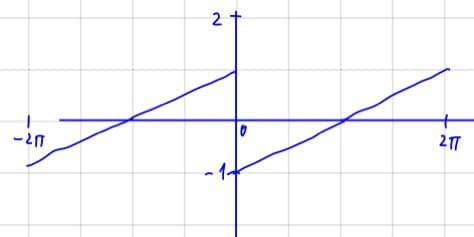
\includegraphics[width=.35\textwidth]{Dateien/06/06Fourier1.jpg}
\end{center}
Wir berechnen die verschiedenen Koeffizienten:
\begin{itemize}
    \item $a_0$:
    \begin{equation*}
        a_0=\frac{1}{\pi}\int_0^{2\pi}\frac{x-\pi}{\pi}dx=\frac{1}{\pi}\BracedIn{\frac{(2\pi)^2}{2\pi}-\frac{2\pi^2}{\pi}}=2-2=0
    \end{equation*}
    \item $a_k$ für $k\neq0$:
    \begin{align*}
        a_k&=\frac{1}{\pi}\int_0^{2\pi}\frac{x-\pi}{\pi}\cos(kx)dx=\frac{1}{\pi^2}\frac{\cos(k x) + k x \sin(k x)}{k^2}\big|_0^{2\pi}-\frac{1}{k\pi}\sin(kx)\big|_0^{2\pi}\\
        &=\frac{1}{(k\pi)^2}(\cos(2\pi k)-\cos(0))=\frac{1}{(k\pi)^2}(1-1)=0
    \end{align*}
    \item Dass $a_k=0\,\forall k\in \mathbb{N}$ ist, hätte uns auch auffallen können, denn $f$ ist bzgl. $x=\pi$ symmetrisch ($f(-(x-\pi))=\frac{-x+\pi-\pi}{\pi}=-\frac{x}{\pi}=-f(x-\pi)$.
    \item $b_k$:
    \begin{align*}
        b_k&=\frac{1}{\pi}\int_0^{2\pi}\frac{x-\pi}{\pi}\sin(kx)dx\\
        &=\frac{1}{\pi^2}\int_0^{2\pi}x\sin(kx)dx-\frac{1}{\pi}\int_0^{2\pi}dx\\
        \overset{\tx{p. Int.}}&{=}\frac{1}{\pi^2}\BracedInSqr{x\BracedIn{-\frac{1}{k}\cos(kx)}}_0^{2\pi}+\frac{1}{k\pi^2}\int_0^{2\pi}\cos(kx)dx+\BracedInSqr{\frac{1}{k\pi}\cos(kx)}_0^{2\pi}\\
        &=-\frac{2}{k\pi}\cos(2\pi k)+\BracedInSqr{\frac{1}{k^2\pi^2}\sin(kx)}_0^{2\pi}+\frac{1}{k\pi}(1-1)\\
        &=-\frac{2}{k\pi}
    \end{align*}
\end{itemize}
Somit ist unsere Fourierreihe
\begin{equation}
    F(f)(x)=-\frac{2}{\pi}\sum_{k=1}^\infty\frac{1}{k}\sin(kx)\quad\forall x\in\mathbb{R}\setminus\MengeDirekt{2\pi n\,(n\in\mathbb{Z})}.
\end{equation}
Achtung! Hier liegt keine \textit{punktweise} Konvergenz $\forall x$ mehr vor! Dies ist der Grund, weshalb wir den neuen Konvergenzbegriff eingeführt hatten.\\
Beispiel: Für $x=0$ ist $f(0)=-1$, aber $F(f)(0)=0$.\\
Gilt hier die parsevalsche Gleichung?\\
Wir haben
\begin{equation*}
    c_k=\Cases{0&k=0\\-\frac{b_k}{2}i\,&k>0\\\frac{b_{-k}}{2}i&k<0},\quad c_k=\overline{c_{-k}}.
\end{equation*}
Somit ist
\begin{equation*}
    \sum_{-\infty}^\infty\Abs{c_k}^2=2\sum_{k=1}^\infty\Abs{c_k}=2\sum_{k=1}^\infty\frac{1}{k^2\pi^2}\overset{\footnote{Es ist $\sum_{k=1}^\infty\frac{1}{k^2}=\frac{\pi^2}{6}$. Würden wir das jetzt nicht als 'Überprüfung' verwenden, würde dies durch die parseval'sche Gleichung auch gezeigt werden.}}{=}\frac{2}{\pi^2}\frac{\pi^2}{6}=\frac{1}{3}.
\end{equation*}
Andererseits ist
\begin{align*}
    \Norm{f}_2^2&=\frac{1}{2\pi}\int_0^{2\pi}\Abs{f(x)}^2dx=\frac{1}{2\pi}\int_0^{2\pi}\BracedIn{\frac{x-\pi}{\pi}}^2dx\\
    \overset{z=x-\pi}&{=}\frac{1}{2\pi^3}\int_{-\pi}^\pi z^2dz=\frac{1}{2\pi^3}\frac{1}{3}(\pi^3-(-\pi)^3)=\frac{1}{3}.\,\checkmark
\end{align*}
\end{Beispiel}
\begin{Beispiel}
{Die Sprungfunktion (2/3)}
Wichtig für die Regeltechnik ist die Sprungfunktion
\begin{equation*}
    f(x)=\Cases{1&\tx{für }x\in[0,\pi)\\-1\,&\tx{für }x\in[\pi,2\pi]}.
\end{equation*}
\begin{center}
    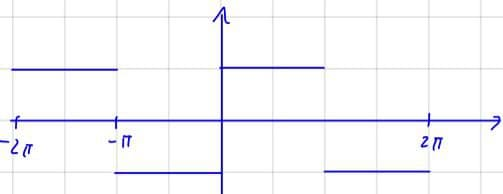
\includegraphics[width=.35\textwidth]{Dateien/06/06Fourier2.jpg}
\end{center}
Diese ist wieder punktsymmetrisch um $x=\pi$, es ist $f(-(x-\pi))=-f(x-\pi)$.\\
Somit sind $a_k=0\,\forall k\in \mathbb{N}$, wir müssen nur $b_{k}$ berechnen:
\begin{align*}
    b_k&=\frac{1}{\pi}\int_0^{2\pi}f(x)\sin(kx)dx=\frac{1}{\pi}\int_0^{\pi}\sin(kx)dx-\frac{1}{\pi}\int_\pi^{2\pi}\sin(kx)dx\\
    &=\frac{1}{\pi}\BracedInSqr{-\frac{1}{k}\cos(kx)}_0^\pi-\frac{1}{\pi}\BracedInSqr{-\frac{1}{k}\cos(kx)}_\pi^{2\pi}\\
    &=\frac{1}{k\pi}-\frac{1}{k\pi}\cos(k\pi)+\frac{1}{k\pi}-\frac{1}{k\pi}\cos(k\pi)\\
    &=\frac{2}{k\pi}(1-(-1)^k).
\end{align*}
Für gerade $k$ ist $b_k=0$, sodass wir gefahrlos $k=2j-1$ substituieren können:
\begin{equation*}
    b_k=b_{2j-1}=\frac{2}{\pi(2j-1)}(1+1)=\frac{4}{(2j-1)\pi}.
\end{equation*}
Damit ist die Fourierreihe
\begin{equation*}
    F(f)(x)=\frac{4}{\pi}\sum_{k=1}^\infty\frac{1}{2k-1}\sin((2k-1)x)\quad\forall x\in\mathbb{R}\setminus\MengeDirekt{2\pi n\,(n\in\mathbb{Z})}.
\end{equation*}
\end{Beispiel}
\red{Achtung: Für das folgende Beispiel betrachten wir das Skalarprodukt auf $[-\pi,\pi)$, also um $\pi$ nach links verschoben! Die Rechnungen sind analog, aber die Integralgrenzen anders.}
\begin{Beispiel}
{Weitere Reihe und Anwendung der parsevalschen Gleichung (3/3)}
Wir betrachten $g(x)=(x-\pi)^2$ auf $[0,2\pi)$. Dies können wir auch von Anfang an um $\pi$ zum Ursprung verschieben, sodass wir $f(x)=x^2$ auf $[-\pi,\pi)$ betrachten.
\begin{center}
    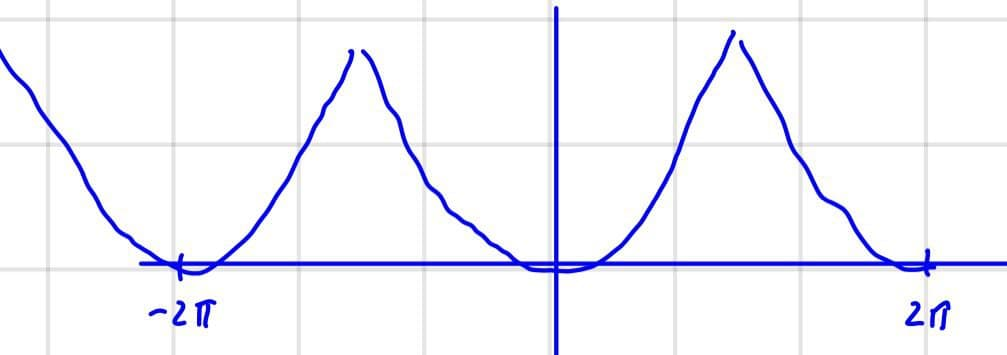
\includegraphics[width=.35\textwidth]{Dateien/06/06Fourier3.jpg}
\end{center}
Diese Funktion ist $2\pi$-periodisch. Zudem sehen wir, dass $f(x)=f(-x)$ ist, sie ist also symmetrisch. Daher sind $b_k=0\,\forall k\in\mathbb{N}$.\\
Wir berechnen also:
\begin{equation*}
    a_0=\frac{1}{\pi}\int_{-\pi}^\pi x^2dx=\frac{2\pi^3}{3\pi}=\frac{2\pi^2}{3}.
\end{equation*}
Aufgrund der Periodizität gilt
\begin{equation*}
    \int_0^\pi f(x)\cos(kx)dx\overset{x\to-x}{=}-\int_0^\pi f(-x)\cos(-kx)dx\overset{\footnote{Symmetrie und Vertauschen der Integralgrenzen}}{=}\int_{-\pi}^0f(x)\cos(kx)dx.
\end{equation*}
Daher haben wir:
\begin{align*}
    a_k&=\frac{1}{\pi}\int_{-\pi}^0 f(x)\cos(kx)dx+\frac{1}{\pi}\int_0^\pi f(x)\cos(kx)dx=\frac{2}{\pi}\int_0^\pi x^2\cos(kx)dx\\
    \overset{\tx{p. Int.}}&{=}\frac{2}{\pi}\BracedInSqr{x^2\frac{1}{k}\sin(kx)}_0^\pi-\frac{2}{\pi}\int_0^\pi\frac{2 x}{k}\sin(kx)dx\\
    \overset{\tx{p. Int.}}&{=}\frac{2}{\pi}\BracedInSqr{x^2\frac{1}{k}\sin(kx)-\BracedIn{-\frac{2}{k^2}x\cos(kx)}-\frac{2\sin(kx)}{k^3}}_0^\pi\\
    &=\frac{4}{\pi k^2}\BracedInSqr{\pi\cos(k\pi)-0\cos(0)}=\frac{4\cos(k\pi)}{k^2}\\
    &=\frac{4}{k^2}(-1)^k.
\end{align*}
Da $f(x)$ stückweise stetig differenzierbar und stetig ist, konvergiert die Fourierreihe 
\begin{equation*}
    (F_n(f))_n=\frac{3\pi^2}{3\cdot2}+\sum_{k=1}^n\frac{4}{k^2}(-1)^k\cos(kx)
\end{equation*}
gleichmäßig gegen $f(x)$, d. h. $\lim_{n\to\infty}(F_n(f))_n=f(x)$ bzw.
\begin{equation*}
    x^2=\frac{\pi^2}{3}+\sum_{k=1}^\infty \frac{4}{k^2}(-1)^k\cos(kx).
\end{equation*}
Betrachten wir nun die Punkte $x=0$ und $x=\pi$, können wir Informationen über die Reihe gewinnen. Hier haben wir (mit $\cos(0k)=1$ und $\cos(k\pi)=(-1)^k$):
\begin{alignat*}{3}
x=0:&\,&f(0)=F(f)(0)\iff 0&=\frac{\pi^2}{3}+\sum_{k=1}^\infty\frac{(-1)^k}{k^2}4\cos(0)\iff \sum_{k=1}^\infty\frac{(-1)^{k+1}}{k^2}=\frac{\pi^2}{12}.\\
x=\pi:&&\pi^2&=\frac{\pi^2}{3}+\sum_{k=1}^\infty\frac{(-1)^k}{k^2}4(-1)^k\iff \sum_{k=1}^\infty\frac{1}{k^2}=\frac{\pi^2}{6}.
\end{alignat*}
Mit diesem Ansatz haben wir also mal eben das \href{https://de.wikipedia.org/wiki/Basler_Problem}{Basler Problem} gelöst, was die Frage nach der reziproken Summe aller Quadratzahlen stellte!\\
Für noch weitere Informationen können wir die Parsevalsche Gleichung verwenden:
\begin{equation*}\label{eq:06HilfeParseval}
    \Norm{f}_2^2=\sum_{k=-\infty}^\infty\Abs{c_k}^2,\tx{ es ist }c_k=\Cases{a_0/2\,&k=0\\a_k/2&k>0\\a_{-k}/2&k<0}.
\end{equation*}
Somit ergibt sich
\begin{align*}
    \Norm{f}_2^2&=\frac{1}{2\pi}\int_{-\pi}^\pi f(x)\overline{f(x)}dx=\frac{2\pi^5}{2\pi 5}\\
    \sum_{-\infty}^\infty \Abs{c_k}^2&=\sum_{k=-\infty}^{-1}\Abs{\frac{4}{k^2}(-1)^k\frac{1}{2}}^2+\Abs{\frac{\pi^2}{3}}^2+\sum_{k=1}^\infty\Abs{\frac{4}{k^2}(-1)^k\frac{1}{2}}^2=\frac{\pi^4}{9}+8\sum_{k=1}^\infty\frac{1}{k^4}\\
    \overset{\eqref{eq:06HilfeParseval}}{\iff}\frac{\pi^4}{5}&=\frac{\pi^4}{9}+8\sum_{k=1}^\infty\frac{1}{k^4}\\
    \iff\sum_{k=1}^\infty\frac{1}{k^4}&=\frac{\pi^4}{8\cdot 5}-\frac{\pi^4}{8\cdot9}=\pi^4\frac{9-5}{8\cdot 45}=\frac{\pi^4}{90},
\end{align*}
ein weiteres bemerkenswertes Ergebnis!
\end{Beispiel}
\Tipps{7}{
\begin{enumerate}
    \item Wenn ihr hier mit der genauen Definition offener Mengen herangeht, sollte der Beweis fix gemacht und logisch sein.
    \item Was bedeutet es mathematisch und anschaulich, wenn $a$ der Grenzwert der Folge ist? Denkt dran, dass jede offene Überdeckung auch der Grenzwert enthalten sein muss.\\
    Für $b)$ und $c)$ gibt es einen Satz, der euch das Leben leichter macht.\\
    Bei $c)$ benötigt ihr vermutlich noch einen Satz über das Bild stetiger Funktionen.
    \item Geschickte Abschätzungen sind gefragt. Schaut euch unsere Beispiele zu Funktionenfolgen an. Bei b) bietet sich für die punktweise Konvergenz eine Fallunterscheidung der Funktion an - welche unterschiedlichen Fälle werden durch das Maximum hervorgerufen? Für die gleichmäßige Konvergenz ist es hilfreich, ein bisschen herumzuprobieren, welche Folgen problematisch für $x$ sein könnten (guckt euch den Term im Betrag gut an!).\\
    Die Integrale dann einfach stumpf ausrechnen (das sollte mit den Intervallen aus der Fallunterscheidung gut möglich sein).
    \item Zu dieser Aufgabe gibt es nicht viel an Tipps zu geben - ein paar Definitionen einsetzen hier, ein paar Integrale dort, und schon seid ihr fertig. Verrechnet euch bloß nicht ;)
    \item a) ist eine Aufgabe, deren Ergebnis sehr wichtig ist. Mit den Definitionen sollte sie schnell gemacht sein.\\
    Zu b): Für die beiden Bereiche mit $y\lessgtr0$ könnt ihr jeweils eine Potentialfunktion durch Integration bestimmen. Beachtet, dass, wenn ihr über $x$ integriert, die Integrations'konstante' noch von $y$ abhängig sein kann!\\
    Zu diesen Themen kommen unsere Notizen leider erst nächste Woche.
\end{enumerate}}